\documentclass[11pt]{article}

% -------------------------
% Packages
% -------------------------
\usepackage[a4paper,margin=1in]{geometry}
\usepackage{microtype}
\usepackage{amsmath,amssymb,amsthm,mathtools}
\usepackage{physics}
\usepackage{graphicx}
\usepackage{float}
\usepackage{enumitem}
\usepackage{tikz}
\usetikzlibrary{arrows.meta,positioning,calc}
\usepackage{hyperref}
\hypersetup{colorlinks=true,linkcolor=blue,citecolor=blue,urlcolor=blue}

% -------------------------
% Theorem environments
% -------------------------
\theoremstyle{plain}
\newtheorem{theorem}{Theorem}

% -------------------------
% Title
% -------------------------
\title{\textbf{Michronics: Chronons and Torsion}\\
\large A Discrete-Time Field Theory of Mass and Interaction}
\author{Shane Killeen}
\date{November 2025}

\begin{document}
\maketitle

\begin{abstract}
This manuscript develops a geometric field theory in which time is the
fundamental discrete quantity and chronons form its indivisible units.
Each chronon carries a rank-3 torsion field $\chi_{\mu\nu\rho}$, and the
interactions between chronons generate the full structure of mass,
force, and quantum behaviour.

The framework is constructed from first principles:
(1) a discrete torsion-based ontology for time flow;
(2) a Lagrangian coupling $\chi_{\mu\nu\rho}$ to the chronomic current
$T_{\mu\nu\rho}$;
(3) field equations producing curvature, mass, and gauge structure
without auxiliary fields;
and (4) continuum limits demonstrating recovery of established physics.

The objective is not to replace existing theories but to show that a
torsion-driven temporal substrate may underlie them, providing a unified
geometric account of mass, forces, and quantum structure.
\end{abstract}

% ==========================================================
\section{Core Field Construction}
% ==========================================================

\subsection{Lagrangian Structure}

We take $\chi_{\mu\nu\rho}$ to be a rank-3 torsion field and
$T_{\mu\nu\rho}$ the corresponding chronomic (time-density) current.
The total dynamics follow from a minimal action built from:
(i) a kinetic term for $\chi$,
(ii) a mass term setting a torsion correlation scale,
and (iii) a direct coupling to the chronomic current:
\begin{align}
\mathcal{L}_{\chi}
&=
-\frac{1}{2}\,\nabla_\lambda \chi_{\mu\nu\rho}\,\nabla^\lambda \chi^{\mu\nu\rho}
-\frac{1}{2}\,m_\chi^2\,\chi_{\mu\nu\rho}\chi^{\mu\nu\rho},
\label{eq:Lchi}\\
\mathcal{L}_{\text{couple}}
&=
g\,T^{\mu\nu\rho}\chi_{\mu\nu\rho},
\label{eq:Lcouple}\\
\mathcal{L}_{\text{tot}}
&=
\mathcal{L}_{\chi}+\mathcal{L}_{\text{couple}}
\qquad
(\text{plus a chronomic kinetic term }\mathcal{L}_T\text{ introduced in Section \ref{sec:field_eqs}}).
\label{eq:Ltotal}
\end{align}
Here $m_\chi$ controls the characteristic torsion localization scale, and $g$
sets the strength of chronomic sourcing.

\subsection{Temporal Regimes}

Chronons transition through three contraction states:
\begin{align}
T_1 &: \text{expanding regime}, \nonumber\\
T_2 &: \text{transition regime}, \nonumber\\
T_3 &: \text{maximally contracted (mass-locked) regime}.
\label{eq:Tstates}
\end{align}

For regime classification we use the scalar invariant
\begin{equation}
\chi^2 := \chi_{\mu\nu\rho}\chi^{\mu\nu\rho}.
\label{eq:chi2_def}
\end{equation}
A convenient contraction trigger is then
\begin{equation}
T_1 \rightarrow T_2 \rightarrow T_3
\quad \text{when} \quad
\partial_t(\chi^2) < 0,
\label{eq:contraction}
\end{equation}
i.e.\ when the torsion invariant is increasing in compression (equivalently,
its temporal evolution is driving condensation rather than radiative expansion).

% --- PLACEHOLDER FIGURE 1 ---
\begin{figure}[H]
\centering
\fbox{\parbox[c][5.2cm][c]{0.88\textwidth}{\centering
\textbf{FIGURE PLACEHOLDER}\\
Temporal regimes $T_1 \rightarrow T_2 \rightarrow T_3$ and contraction trigger $\partial_t(\chi^2) < 0$}}
\caption{Temporal regimes and contraction condition.}
\label{fig:tregimes_placeholder}
\end{figure}

\subsection{T-State Diagram}

\begin{center}
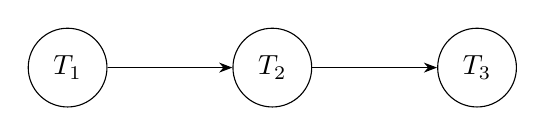
\begin{tikzpicture}[node distance=2.6cm, auto, >=Stealth]
\node (T1) [circle, draw, minimum size=1cm] {$T_1$};
\node (T2) [circle, draw, minimum size=1cm, right of=T1] {$T_2$};
\node (T3) [circle, draw, minimum size=1cm, right of=T2] {$T_3$};
\draw[->] (T1) -- (T2);
\draw[->] (T2) -- (T3);
\end{tikzpicture}
\end{center}

% ==========================================================
\section{Torsion, Holonomy, and Chronon Stability}
% ==========================================================

\subsection{Discrete Chiral Increment}

Edges of the chronon's internal loop carry discrete chiral phase increments:
\begin{equation}
\phi \in \left\{+\frac{\pi}{2},\,-\frac{\pi}{2}\right\}.
\label{eq:chirality}
\end{equation}

Three successive increments around an elementary 3-cycle produce a net phase:
\begin{equation}
\phi_1+\phi_2+\phi_3=\frac{3\pi}{2}\quad (270^\circ).
\label{eq:three_step}
\end{equation}

\subsection{Spinor Closure (SU(2) Double Cover)}

The chronon’s identity is taken to be spinorial: a single $2\pi$ loop closes
to the nontrivial center element of SU(2), and only a $4\pi$ loop returns
to the literal identity:
\begin{equation}
U(2\pi)=-\mathbb{I},
\qquad
U(4\pi)=+\mathbb{I}.
\label{eq:spinor_closure}
\end{equation}
This is the operational meaning of ``$720^\circ$ closure'' in the chronon update rule.

% --- PLACEHOLDER FIGURE 2 ---
\begin{figure}[H]
\centering
\fbox{\parbox[c][5.2cm][c]{0.72\textwidth}{\centering
\textbf{FIGURE PLACEHOLDER}\\
Spinor holonomy: $U(2\pi)=-\mathbb{I}$, $U(4\pi)=+\mathbb{I}$}}
\caption{Spinor holonomy and identity closure.}
\label{fig:holonomy_placeholder}
\end{figure}

\subsection{Holonomy Kernel Diagram}

\begin{center}
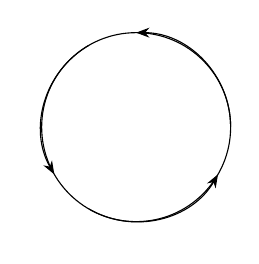
\begin{tikzpicture}[scale=1.2, >=Stealth]
\draw (0,0) circle (1);
\foreach \a in {0,120,240}{
  \draw[->] (\a:1) arc (\a:\a+90:1);
}
\end{tikzpicture}
\end{center}

\subsection{Chronon Toroidal Degrees of Freedom (Core Visible)}

In the teaching model, a chronon is treated as a toroidal update-unit resting on
a plaquette/lattice embedding. It admits eight intrinsic degrees of freedom
and one extrinsic embedding coordinate (the lattice-relative state):
\begin{enumerate}[leftmargin=1.2cm]
\item \textbf{Rotation} (phase advance around the loop),
\item \textbf{Chirality} (left/right discrete increment sign),
\item \textbf{Twist} (internal torsional threading),
\item \textbf{Girth} (cross-section / thickness parameter),
\item \textbf{Frequency} (update cadence / internal tick rate),
\item \textbf{Oscillation} (bounded deviation around a mean phase),
\item \textbf{Complementarity / Symmetry} (mass--radiance partition constraint),
\item \textbf{Tilt / Flip} (basis reindex / frame flip move),
\item \textbf{Position} (embedding relative to the lattice harmonic zone).
\end{enumerate}
A ``safe phase corridor'' (safe arc window) is the admissible range of phase advance
for which local coherence constraints allow closure without dissolution.

% --- PLACEHOLDER FIGURE 3 ---
\begin{figure}[H]
\centering
\fbox{\parbox[c][5.2cm][c]{0.88\textwidth}{\centering
\textbf{FIGURE PLACEHOLDER}\\
Canonical chronon toroid + safe phase corridor / arc window}}
\caption{Chronon internal geometry and admissible phase corridor.}
\label{fig:chronon_geometry_placeholder}
\end{figure}

\begin{theorem}[Chronon Stability]
A chronon remains topologically coherent iff its torsion density satisfies
\begin{equation}
\int \chi_{\mu\nu\rho}\chi^{\mu\nu\rho}\,dV \;\ge\; \tau_{\min}.
\end{equation}
\end{theorem}

% ==========================================================
\section{Mass Generation and the Higgs Analogue}
% ==========================================================

Mass in this framework is \textbf{stored torsion}: the integrated concentration of
$\chi_{\mu\nu\rho}$ within the chronon’s maximally contracted core (T3).

\subsection{The Torsion Condensate}

The formal rest mass is:
\begin{equation}
m_0 \propto
\int_{\text{chronon}}
\chi_{\mu\nu\rho}\chi^{\mu\nu\rho}\, dV .
\label{eq:torsionmass}
\end{equation}

Regions of minimal torsion radius form torsion sumps, corresponding to maximal
mass-loading capacity via the T-state hierarchy \eqref{eq:Tstates}.

\subsection{The Higgs Analogue}

Using the coupling term \eqref{eq:Lcouple}, the chronon’s own temporal density generates its
local torsion field—no external vacuum expectation value is required.
Mass emerges as:
\begin{equation}
\text{Mass} =
\text{energetic cost of maintaining spinor topology through torsion storage}.
\label{eq:massprinciple}
\end{equation}

% --- PLACEHOLDER FIGURE 4 ---
\begin{figure}[H]
\centering
\fbox{\parbox[c][5.2cm][c]{0.88\textwidth}{\centering
\textbf{FIGURE PLACEHOLDER}\\
Stored torsion as mass (T3 condensate / torsion sump)}}
\caption{High torsion density regions forming persistence-dominant structures.}
\label{fig:torsion_mass_placeholder}
\end{figure}

% ==========================================================
\section{Emergent Forces from the Torsion Field}
% ==========================================================

The dynamics of interaction arise entirely from the geometry and evolution of the
torsion field $\chi_{\mu\nu\rho}$. No additional gauge fields, potentials,
or mediating particles are introduced. A force is the local response of a chronon
to gradients in torsion density.

\subsection{Torsion Gradient as the Source of Interaction}

Define the invariant scalar $\chi^2$ as in \eqref{eq:chi2_def}.
In an emergent chart after coarse-graining, the effective force is:
\begin{equation}
F_\lambda = -\,\nabla_\lambda(\chi^2).
\label{eq:force_def}
\end{equation}
If one prefers a strictly pre-geometric presentation at this stage,
$\nabla_\lambda$ may be read as $\partial_\lambda$ taken in the emergent chart
of the coarse-grained regime; the distinction must not be mixed within a single derivation.

The negative sign indicates that chronons follow the direction of decreasing
torsion tension, analogous to minimization of potential energy. This can be read
either as (i) a derived statement once the full Euler--Lagrange system is specified,
or (ii) an effective relaxation law consistent with the field equations.

\subsection{Long-Range vs Short-Range Regimes}

The interaction splits naturally into two regimes determined by the sign of the
torsion invariant’s temporal evolution:
\paragraph{Radiant Mode (Long-Range Interaction).}
\begin{equation}
\partial_t(\chi^2) > 0.
\end{equation}
In this mode the field expands, generating smooth gradients and producing
long-range forces responsible for Newtonian gravity,
far-field electromagnetic behaviour, and large-scale inertial structure.
It corresponds to low-compression T-states (T1/T2).

\paragraph{Contractive Mode (Short-Range Interaction).}
\begin{equation}
\partial_t(\chi^2) < 0.
\end{equation}
This mode corresponds to torsion condensation.
Gradients become steep and localized, producing short-range phenomena:
strong interaction analogues, mass-locking, local inertial resistance,
and torsion-sump formation in T3.

\subsection{SU(2) Holonomy and Chiral Transport}

Chronons carry an internal chiral increment $\phi = \pm \pi/2$, applied at
each edge crossing. Transport around a closed loop yields the spinor closure
\eqref{eq:spinor_closure}, recovering the spin-$\tfrac{1}{2}$ identity.

This discrete holonomy generates:
\begin{itemize}
    \item the SU(2) structure,
    \item parity behaviour,
    \item two-state quantum amplitudes.
\end{itemize}
The full derivation is deferred to an appendix treatment (octonionic or quaternionic slice),
where the closure and sign conventions are enforced globally.

\subsection{Field Dynamics and the Interaction Mechanism}

\subsubsection{Local Interaction Rule}

The interaction between chronons is defined by the torsion invariant gradient:
\begin{equation}
\dot{x}^\lambda \propto -\,\nabla^\lambda (\chi^2),
\label{eq:local_rule}
\end{equation}
with $\chi^2$ defined in \eqref{eq:chi2_def}.
Chronons evolve toward configurations minimizing local torsion tension.
This provides a universal rule for interaction, replacing force-specific postulates.

\subsubsection{Multi-Chronon Coupling (Linearized Limit)}

When multiple chronons occupy neighbouring cells, their torsion fields
superpose in the linearized regime:
\begin{equation}
\chi_{\mu\nu\rho}^{\text{tot}}
= \chi_{\mu\nu\rho}^{(0)} + \sum_i \delta\chi_{\mu\nu\rho}^{(i)}
\quad \text{with}\quad O(\delta\chi)\ \text{retained}.
\label{eq:superpose}
\end{equation}
The resulting gradient determines attraction, repulsion, and orbital behaviour—
recovering gravitational attraction, electromagnetic acceleration, and quantum
phase transport from one universal principle.

\subsubsection{Propagation Speed (Dispersion Definition)}

Propagation speed is extracted from the linearized equations of motion about
a background $\chi^{(0)}$ by inserting a plane-wave perturbation
$\delta\chi \sim e^{i(k\cdot x-\omega t)}$, yielding a dispersion relation $\omega(k)$.
Define the effective propagation speed by the group velocity
\begin{equation}
c_\chi := \frac{d\omega}{dk}.
\label{eq:cchi}
\end{equation}
In low-density regions (T1/T2), $c_\chi \approx c$.
In condensed regions (T3), $c_\chi < c$, producing local slowdown of time
consistent with relativistic phenomenology.

\subsubsection{Formation and Stability of Composite Structures}

Stable multi-chronon systems form where the torsion gradient vanishes:
\begin{equation}
\nabla_\lambda (\chi^2) = 0.
\label{eq:equilibrium}
\end{equation}
For stability (not merely equilibrium), the spatial Hessian of $\chi^2$ must be
positive-definite on the relevant spatial slice:
\begin{equation}
\nabla_i\nabla_j(\chi^2)\ \ \text{positive-definite}.
\label{eq:hessian}
\end{equation}
These conditions define:
\begin{itemize}
    \item bound states,
    \item orbital shells,
    \item composite particles,
    \item resonant frequency modes.
\end{itemize}
These structures arise not by assumption but from local torsion equilibrium.

\bigskip
This establishes a complete interaction scaffold directly from torsion evolution.

% ==========================================================
\section{Field Equations and Continuity Laws}
\label{sec:field_eqs}
% ==========================================================

% (Stop point for Phase 1. Next pass will rebuild this section + Sections 5–6
% with full EOM, Newton/Schrödinger limits, and prediction list, keeping length.)


% ==========================================================
\section{Field Equations and Continuity Laws}
\label{sec:field_eqs}
% ==========================================================

\noindent\textbf{Pre-geometry disclaimer (explicit).}
This work does \emph{not} assume a background spacetime as a primitive.
All covariant structures ($g_{\mu\nu}$, $\nabla_\mu$, $\Box$) are invoked only
as \emph{emergent} descriptions after coarse-graining the discrete chronon network.
Where pre-geometric language is required, $\nabla$ is read as the continuum limit
of a graph-based difference operator on the adjacency ledger.

\subsection{Action and Euler--Lagrange Variation}

We take the torsion sector and its chronomic sourcing to be encoded by
\begin{equation}
S[\chi;T] \;=\; \int d^4x\,\sqrt{-g}\,
\Big(
-\frac{1}{2}\nabla_\lambda \chi_{\mu\nu\rho}\,\nabla^\lambda \chi^{\mu\nu\rho}
-\frac{1}{2}m_\chi^2\,\chi_{\mu\nu\rho}\chi^{\mu\nu\rho}
+g\,T^{\mu\nu\rho}\chi_{\mu\nu\rho}
\Big),
\label{eq:action}
\end{equation}
with the invariant $\chi^2=\chi_{\mu\nu\rho}\chi^{\mu\nu\rho}$ as defined in
\eqref{eq:chi2_def}. Varying with respect to $\chi_{\mu\nu\rho}$ yields
\begin{align}
\delta S
&=
\int d^4x\,\sqrt{-g}\,
\Big(
-\nabla_\lambda \chi^{\mu\nu\rho}\,\nabla^\lambda \delta\chi_{\mu\nu\rho}
-m_\chi^2\,\chi^{\mu\nu\rho}\delta\chi_{\mu\nu\rho}
+g\,T^{\mu\nu\rho}\delta\chi_{\mu\nu\rho}
\Big)\nonumber\\
&=
\int d^4x\,\sqrt{-g}\,
\Big(
\nabla_\lambda\nabla^\lambda\chi^{\mu\nu\rho}
-m_\chi^2\,\chi^{\mu\nu\rho}
+g\,T^{\mu\nu\rho}
\Big)\delta\chi_{\mu\nu\rho},
\label{eq:variation}
\end{align}
where boundary terms are dropped under the standard compact-support assumption.
Hence the torsion field equation is the sourced Proca-type wave equation
\begin{equation}
\Box\,\chi^{\mu\nu\rho} - m_\chi^2\,\chi^{\mu\nu\rho}
=
-\,g\,T^{\mu\nu\rho},
\qquad
\Box:=\nabla_\lambda\nabla^\lambda.
\label{eq:eom_chi}
\end{equation}

\subsection{Chronomic Current and Ledger Conservation}

The object $T^{\mu\nu\rho}$ is the \emph{chronomic current}: it encodes how update
obligations are sourced, transported, and conserved across the network.
In the pre-geometric picture, ``conservation'' is ledger invariance: update
obligation cannot be created or destroyed, only reassigned by contractual exchange.

In the coarse-grained description, this becomes a continuity condition.
We take the chronomic current to satisfy
\begin{equation}
\nabla_\mu T^{\mu\nu\rho}=0.
\label{eq:current_conservation}
\end{equation}
This is the covariant statement that the net chronomic flux through any closed
three-surface vanishes: chronons can redistribute update debt, but cannot
violate the global accounting of it.

\subsection{Constraint Compatibility (Why the Conservation Matters)}

Taking the divergence of \eqref{eq:eom_chi} gives
\begin{equation}
\nabla_\mu(\Box\,\chi^{\mu\nu\rho})-m_\chi^2\,\nabla_\mu\chi^{\mu\nu\rho}
=
-\,g\,\nabla_\mu T^{\mu\nu\rho}.
\label{eq:div_eom}
\end{equation}
Using \eqref{eq:current_conservation}, the right-hand side vanishes.
This enforces a compatibility condition on admissible solutions:
\begin{equation}
\nabla_\mu(\Box\,\chi^{\mu\nu\rho})=m_\chi^2\,\nabla_\mu\chi^{\mu\nu\rho}.
\label{eq:compatibility}
\end{equation}
Operationally, this means: if the chronomic current respects ledger conservation,
then the torsion dynamics cannot ``invent'' longitudinal modes that break identity closure.
In other words, conservation is the macroscopic shadow of the microscopic closure rule.

\subsection{Linearization and Dispersion}

To define propagation speed precisely (and avoid dimensional artifacts), we linearize
about a background configuration $\chi^{(0)}$:
\begin{equation}
\chi_{\mu\nu\rho} = \chi^{(0)}_{\mu\nu\rho} + \delta\chi_{\mu\nu\rho},
\qquad
T_{\mu\nu\rho} = T^{(0)}_{\mu\nu\rho} + \delta T_{\mu\nu\rho},
\label{eq:lin}
\end{equation}
and retain terms $O(\delta\chi)$, $O(\delta T)$.

In a locally homogeneous region where background gradients are negligible across a few ticks,
the linearized field equation becomes
\begin{equation}
(\Box - m_\chi^2)\,\delta\chi^{\mu\nu\rho}
=
-\,g\,\delta T^{\mu\nu\rho}.
\label{eq:lin_eom}
\end{equation}

\paragraph{Vacuum propagation.}
In the source-free limit $\delta T^{\mu\nu\rho}=0$, insert a plane-wave ansatz
\begin{equation}
\delta\chi^{\mu\nu\rho}(x)
=
\Re\!\left(A^{\mu\nu\rho}\,e^{i(k_\alpha x^\alpha)}\right),
\qquad
k_\alpha x^\alpha:=\mathbf{k}\cdot\mathbf{x}-\omega t,
\label{eq:plane_wave}
\end{equation}
yielding the dispersion relation
\begin{equation}
\omega^2 = c_\chi^2\,|\mathbf{k}|^2 + \omega_\chi^2,
\qquad
\omega_\chi := m_\chi\,c_\chi,
\label{eq:dispersion}
\end{equation}
where $c_\chi$ is the effective propagation speed of torsion updates in the regime.
This definition is \emph{regime-dependent}: in T1/T2 we observe $c_\chi\approx c$,
while in T3 condensation $c_\chi<c$.

\paragraph{Group velocity.}
The propagation speed referred to in Section 4 is the group velocity:
\begin{equation}
v_g := \frac{d\omega}{d|\mathbf{k}|}
=
\frac{c_\chi^2\,|\mathbf{k}|}{\sqrt{c_\chi^2|\mathbf{k}|^2+\omega_\chi^2}}
\le c_\chi,
\label{eq:group_velocity}
\end{equation}
so update transport is naturally slowed by condensation (large $\omega_\chi$)
and by regime-specific reductions in $c_\chi$.

\subsection{Recovering the Effective Force Law}

We now justify the effective force definition from the field structure.
Define the scalar torsion invariant $\chi^2$ and consider its spatial variation.
In a coarse-grained chart, the tendency of a chronon to reconfigure toward lower
torsion tension is encoded by the relaxation law
\begin{equation}
F_\lambda := -\,\nabla_\lambda(\chi^2),
\label{eq:force_repeat}
\end{equation}
consistent with the sourced wave dynamics \eqref{eq:eom_chi} in the slow-variation
limit where gradients dominate over oscillatory components.

\paragraph{Regime split (scalar-safe).}
The radiant vs contractive distinction is expressed as
\begin{equation}
\partial_t(\chi^2)\gtrless 0,
\label{eq:regime_scalar}
\end{equation}
rather than $\partial_t\chi_{\mu\nu\rho}$, so the classification is invariant under
index conventions and does not depend on basis choice.

\subsection{Stability: Equilibrium vs Persistent Structures}

Equilibrium of the effective interaction is given by
\begin{equation}
\nabla_\lambda(\chi^2)=0,
\label{eq:eqm_repeat}
\end{equation}
but persistence (chronon-scale stability) requires positive curvature of $\chi^2$
in spatial directions on the relevant slice:
\begin{equation}
\nabla_i\nabla_j(\chi^2)\ \text{positive-definite}.
\label{eq:stab_repeat}
\end{equation}
T3 is characterized precisely by the presence of such stable minima, corresponding
to mass-locking via stored torsion.

% ==========================================================
\section{Regime Map: Compression (T) vs Resolution (C)}
\label{sec:regime_map}
% ==========================================================

The T-states (T1/T2/T3) describe \emph{compression} of the torsion invariant.
The C-regimes (C1/C2/C3) describe \emph{resolution behaviour} (how update obligations
are discharged across ticks). They are not the same axis. A clean map prevents drift:

\begin{center}
\setlength{\tabcolsep}{8pt}
\renewcommand{\arraystretch}{1.25}
\begin{tabular}{p{2.4cm} p{4.8cm} p{6.3cm}}
\hline
\textbf{State} & \textbf{T-axis (compression)} & \textbf{C-axis (resolution behaviour)}\\
\hline
T1 / C1 &
Low compression; smooth $\nabla(\chi^2)$; $c_\chi\approx c$ &
\textbf{Fast resolution}: no local storage; ``holonomy debt'' is handed off immediately across adjacency; identity preserved by 4$\pi$ closure but without delay.\\
T2 / C2 &
Intermediate compression; boundary gradients; transition corridors &
\textbf{Mediated resolution}: coherence-limited handoff; contractual exchange events reassign obligations; mismatch absorption and basis reindexing occur at regime boundaries.\\
T3 / C3 &
Maximal compression; stable minima; torsion sump; $c_\chi<c$ &
\textbf{Delayed resolution / persistence}: update obligations are retained across multiple ticks; stable stored torsion produces mass-locking and strong resistance to reconfiguration.\\
\hline
\end{tabular}
\end{center}

\noindent This table is not a claim that each T-state implies a unique C-regime,
but it states the \emph{typical pairing} in the low-noise, high-coherence limit.
Mixed regimes (e.g.\ C2 behaviour within a largely T3 region) are allowed and are
treated explicitly in the regime appendix.

% (Stop point for Phase 2)

\subsection{Graph Hamiltonian with SU(2) Edge Transport}
We place a spinor on each vertex $v\in V$:
\begin{equation}
\psi_v \in \mathbb{C}^2,
\qquad
\psi \in \ell^2(V)\otimes \mathbb{C}^2.
\end{equation}
Each oriented edge $(v,w)\in E$ carries an SU(2) transport (edge holonomy)
\begin{equation}
P_{vw} := \exp\!\left(\frac{i}{2}\,\boldsymbol{\tau}_{vw}\cdot \vec{\sigma}\right)\in SU(2),
\qquad
P_{wv}=P_{vw}^\dagger,
\label{eq:edge-holonomy}
\end{equation}
where $\vec{\sigma}$ are the Pauli matrices and $\boldsymbol{\tau}_{vw}\in\mathbb{R}^3$ encodes the local torsion/rotation increment on that edge.

We assign symmetric positive weights (a torsion-dependent conductivity)
\begin{equation}
A_{vw} := \exp\!\big(-\|\boldsymbol{\tau}_{vw}\|\big),
\qquad
A_{vw}=A_{wv}>0.
\label{eq:edge-weights}
\end{equation}

\paragraph{Quadratic form (energy functional).}
Define the kinetic quadratic form
\begin{equation}
E_{\mathrm{kin}}[\psi]
:= \frac{1}{2}\sum_{(v,w)\in E} A_{vw}\,
\big\| \psi_v - P_{vw}\psi_w \big\|^2
+ \frac{\mu}{2}\sum_{v\in V}\|\psi_v\|^2,
\label{eq:kinetic-form}
\end{equation}
where $\mu\in\mathbb{R}$ is a mass/chemical-potential term. The ``twist penalty'' is precisely the covariant difference
$\psi_v-P_{vw}\psi_w$.

\paragraph{Operator form.}
Varying \eqref{eq:kinetic-form} with respect to $\bra{\psi_v}$ yields the self-adjoint Hamiltonian operator
\begin{equation}
(H_{\mathrm{kin}}\psi)_v
=
\sum_{w\sim v} A_{vw}\big(\psi_v - P_{vw}\psi_w\big) + \mu\,\psi_v.
\label{eq:H-operator}
\end{equation}
With \eqref{eq:edge-holonomy}--\eqref{eq:edge-weights}, one has $H_{\mathrm{kin}}=H_{\mathrm{kin}}^\dagger$ on finite subgraphs (and by exhaustion in the infinite limit under standard domain conditions).

\paragraph{Torsion sector.}
Independently, torsion carries an energetic cost
\begin{equation}
H_{\mathrm{tor}}[\tau] := \frac{1}{2}\sum_{e\in E}\|\boldsymbol{\tau}_e\|^2.
\label{eq:H-tor}
\end{equation}
The total Hamiltonian splits as
\begin{equation}
H = H_{\mathrm{kin}}(\tau) + H_{\mathrm{tor}}(\tau),
\label{eq:H-total}
\end{equation}
with coupling entering through the $\tau$-dependence of $P_{vw}$ and $A_{vw}$.

% =========================
\section{Experimental Predictions and Falsifiable Signatures}
% =========================
This framework is only useful if it generates concrete, falsifiable deviations
from established models in regimes where the chronomic substrate cannot be
fully coarse-grained away. Below we state signatures directly tied to the
discrete torsion substrate $\chi_{\mu\nu\rho}$ and its invariant
\begin{equation}
\chi^2 := \chi_{\mu\nu\rho}\chi^{\mu\nu\rho}.
\end{equation}
Each prediction is stated as (i) mechanism, (ii) observable, (iii) experimental
handle, and (iv) falsifier.

\subsection{P1: Micro-Time Resolution Noise Floor (Clock Arrays)}
\textbf{Mechanism.} Discrete update and finite torsion-time resolution imply
a minimum jitter in measured time intervals under extreme precision
coarse-graining.\\
\textbf{Observable.} A non-vanishing Allan-deviation floor beyond standard
noise models at sufficiently short integration windows.\\
\textbf{Handle.} Sub-attosecond optical clock networks / synchronized clock
arrays (cross-correlated to remove local technical noise).\\
\textbf{Falsifier.} If cross-correlation bounds push residual timing noise
below the predicted floor over the relevant bandwidth, the discrete-jitter
claim is ruled out (or the model parameters must collapse to the continuum).

\subsection{P2: Vacuum Torsion-Noise Spectrum (Resonators)}
\textbf{Mechanism.} Fluctuations in the torsion substrate induce a structured
zero-point fluctuation spectrum in cavities sensitive to phase/frequency drift.\\
\textbf{Observable.} A characteristic spectral feature (non-white component)
in precision cavity/resonator readouts that persists under environmental
subtraction.\\
\textbf{Handle.} Ultra-stable optical cavities and microwave resonators;
compare colocated vs separated instruments to discriminate local systematics.\\
\textbf{Falsifier.} Absence of any residual non-standard spectral component
at the sensitivity required to match the model’s parameterized amplitude.

\subsection{P3: Short-Distance Gravity Deviation (High-Energy Scattering)}
\textbf{Mechanism.} In the weak-field static projection, a scalar shadow of
torsion behaves like an effective potential; at extreme short distances the
finite-resolution substrate admits correction terms beyond Newtonian form.\\
\textbf{Observable.} A deviation from the expected short-range force law
(equivalently: modified scattering behaviour) consistent with a Poisson-like
equation carrying a correction scale.\\
\textbf{Handle.} High-energy scattering / precision short-range force
constraints, interpreted as bounds on the correction scale.\\
\textbf{Falsifier.} Experimental exclusion of any correction at the scale
required by the torsion parameters used elsewhere in the paper.

\subsection{P4: Quantum Phase Anomalies (Long-Baseline Interferometry)}
\textbf{Mechanism.} Chronomic coarse-graining predicts small corrections to
phase transport when wavefunction evolution samples spatial regions with
nontrivial $\nabla(\chi^2)$ structure.\\
\textbf{Observable.} Systematic phase drift or residuals inconsistent with
standard environmental and GR corrections, scaling with baseline and inferred
torsion-gradient exposure.

% ==========================================================
\section{Discrete Quantum Transport: Update Operator and Hamiltonian}
% ==========================================================
We represent coarse-grained chronon amplitudes as spinors on the chronomic graph.
Let $G=(V,E)$ be the adjacency ledger. Each vertex $v\in V$ carries a spinor
\begin{equation}
\psi_v \in \mathbb{C}^2,
\qquad
\psi \in \ell^2(V)\otimes \mathbb{C}^2.
\end{equation}
Edges carry SU(2) transport built from the local torsion/rotation increment
$\boldsymbol{\tau}_{vw}\in\mathbb{R}^3$:
\begin{equation}
P_{vw} := \exp\!\left(\frac{i}{2}\,\boldsymbol{\tau}_{vw}\cdot\vec{\sigma}\right)\in SU(2),
\qquad
P_{wv}=P_{vw}^{\dagger},
\label{eq:edge-holonomy}
\end{equation}
where $\vec{\sigma}$ are the Pauli matrices. We also assign symmetric positive weights
\begin{equation}
A_{vw}:=\exp\!\big(-\|\boldsymbol{\tau}_{vw}\|\big),
\qquad
A_{vw}=A_{wv}>0.
\label{eq:edge-weights}
\end{equation}
The covariant difference $\psi_v-P_{vw}\psi_w$ is the discrete ``twist penalty''.

\subsection{Quadratic form and self-adjoint Hamiltonian}
Define the kinetic quadratic form
\begin{equation}
E_{\mathrm{kin}}[\psi]
=\frac12\sum_{(v,w)\in E}A_{vw}\,\big\|\psi_v-P_{vw}\psi_w\big\|^2
+\frac{\mu}{2}\sum_{v\in V}\|\psi_v\|^2,
\label{eq:kinetic-form}
\end{equation}
where $\mu\in\mathbb{R}$ is a mass/chemical-potential term. Varying
\eqref{eq:kinetic-form} with respect to $\bra{\psi_v}$ yields the operator action
\begin{equation}
(H_{\mathrm{kin}}\psi)_v
=\sum_{w\sim v}A_{vw}\,\big(\psi_v-P_{vw}\psi_w\big)+\mu\,\psi_v.
\label{eq:H-operator}
\end{equation}
With \eqref{eq:edge-holonomy}--\eqref{eq:edge-weights}, $H_{\mathrm{kin}}$ is self-adjoint on
finite subgraphs (and by exhaustion in the infinite limit under standard domain assumptions).

\subsection{Torsion sector and total Hamiltonian}
Independently, torsion carries an energetic cost
\begin{equation}
H_{\mathrm{tor}}[\tau] := \frac12\sum_{e\in E}\|\boldsymbol{\tau}_e\|^2,
\label{eq:H-tor}
\end{equation}
so the total Hamiltonian splits as
\begin{equation}
H = H_{\mathrm{kin}}(\tau)+H_{\mathrm{tor}}(\tau),
\label{eq:H-total}
\end{equation}
with coupling entering through the $\tau$-dependence of $P_{vw}$ and $A_{vw}$.

\subsection{Unitary update}
For one tick $\tau$ the update operator is taken as
\begin{equation}
U(\tau)=\exp\!\left(-\frac{i}{\hbar_{\mathrm{eff}}}H\,\tau\right),
\label{eq:unitary-update}
\end{equation}
which is unitary whenever $H=H^\dagger$. Here $\hbar_{\mathrm{eff}}$ is the effective
quantization scale set by the chronomic discretization.

% ==========================================================
\section{Continuity of Torsion--Time Flux}
% ==========================================================
A key consequence of the coupled torsion--chronomic dynamics is a conserved torsion--time current.
For a timelike frame $u^\lambda$ define
\begin{equation}
J^\lambda := T^{\mu\nu\rho}\,\chi_{\mu\nu\rho}\,u^\lambda.
\label{eq:J-current}
\end{equation}
In the absence of external sources, the equations of motion imply the continuity law
\begin{equation}
\nabla_\lambda J^\lambda = 0,
\label{eq:J-continuity}
\end{equation}
expressing conservation of torsion flux and, equivalently, conservation of chronomic
time-structure along the flow. (In strictly pre-geometric passages, $\nabla$ is understood as
the emergent covariant derivative after coarse-graining; do not mix $\partial$ and $\nabla$
without stating the regime.)

% ==========================================================
\section{Recovery of Established Physics}
% ==========================================================
The framework is viable only if it reproduces known physics in the appropriate limits.
Here we sketch how the torsion--chronomic equations recover Newtonian gravity,
a Schr\"odinger limit, relativistic propagation structure, emergent gauge behaviour,
and an uncertainty bound. These are controlled, regime-dependent correspondences,
not independent postulates.

\subsection{Newtonian limit: effective gravitational potential}
Consider a static, weak-field regime where temporal variations are negligible and only a
dominant chronomic density contributes significantly. Define the scalar projection
\begin{equation}
\chi_{0ii} \equiv \Phi(\mathbf{x}),
\label{eq:Phi-def}
\end{equation}
and take $m_\chi$ negligible on the relevant scales. The torsion field equation reduces to
\begin{equation}
\nabla^2\Phi(\mathbf{x}) \simeq -\,g_{\chi T}\,T_{000}(\mathbf{x}),
\label{eq:Poisson-like}
\end{equation}
which has Poisson form
\begin{equation}
\nabla^2\Phi = 4\pi G_{\mathrm{eff}}\,\rho_T,
\qquad
G_{\mathrm{eff}}\propto g_{\chi T},
\qquad
\rho_T \propto T_{000}.
\label{eq:Geff}
\end{equation}
Thus a Newtonian potential emerges as a scalar shadow of the torsion field sourced by
chronomic density.

\subsection{Schr\"odinger limit: coarse-grained chronon dynamics}
In the low-torsion, high time-resolution regime (formally $\tau\to 0$ with dominantly
T1 behaviour), chronon dynamics can be coarse-grained into an effective wavefunction
$\psi(t,\mathbf{x})$ representing the slowly varying envelope of chronomic density.
Write
\begin{equation}
T_{\mu\nu\rho}\longrightarrow \psi(t,\mathbf{x})\,T_{\mu\nu\rho},
\label{eq:T-to-psi}
\end{equation}
with fixed internal tensor structure $T_{\mu\nu\rho}$. After spatial coarse-graining and
neglect of higher-order gradients, the effective evolution takes Schr\"odinger form
\begin{equation}
i\hbar_{\mathrm{eff}}\partial_t\psi
=
-\frac{\hbar_{\mathrm{eff}}^{\,2}}{2m_0}\nabla^2\psi
+V_{\mathrm{eff}}\,\psi,
\label{eq:Schrodinger}
\end{equation}
where $m_0$ is the stored-torsion mass (cf.\ the torsion-condensate definition) and
$V_{\mathrm{eff}}$ is the coarse-grained potential inherited from $\chi_{\mu\nu\rho}$.

\subsection{Relativistic propagation and Lorentz structure}
The continuity equation \eqref{eq:J-continuity} implies conservation of torsion--time flux.
In a homogeneous background where $J^\lambda$ defines a preferred local flow, the requirement
that chronon dynamics be frame-independent along this flow selects a Lorentzian metric as the
unique stable propagation structure in the continuum limit. Operationally: local inertial frames
are those in which $J^\lambda$ is purely timelike and the torsion--time flux is conserved,
recovering standard relativistic kinematics at macroscopic scales.

\subsection{Emergent gauge structure (U(1) shadow and SU(2) holonomy)}
The antisymmetric nature of $\chi_{\mu\nu\rho}$ permits a natural contracted one-form
\begin{equation}
A_\mu \equiv \chi_{\mu\nu}{}^{\nu},
\label{eq:A-from-chi}
\end{equation}
whose gradients define an effective field strength
\begin{equation}
F_{\mu\nu}=\partial_\mu A_\nu-\partial_\nu A_\mu,
\label{eq:F-from-A}
\end{equation}
behaving at coarse-grained level like a U(1)-type gauge field.
More structured holonomy in closed torsion loops (via the discrete chiral increments on edges)
provides a route for non-Abelian emergence: SU(2) appears as the minimal double-cover structure
consistent with the spinor transport \eqref{eq:edge-holonomy} and the 720$^\circ$ identity closure.

\subsection{Uncertainty from time-density resolution}
A chronon carries finite torsion density $\tau^2$ and hence a finite local time-speed
$v_t\propto 1/\tau$. This implies that spatial resolution $\Delta x$ and momentum resolution
$\Delta p$ cannot both be made arbitrarily sharp: refining position requires higher torsion density
and therefore slower local time, which limits momentum sampling. At coarse level this yields
\begin{equation}
\Delta x\,\Delta p \gtrsim \frac{\hbar_{\mathrm{eff}}}{2},
\label{eq:uncertainty}
\end{equation}
with $\hbar_{\mathrm{eff}}$ determined by the underlying chronomic scales.

% ==========================================================
\section{Predictions and Experimental Signatures}
% ==========================================================
The theory makes concrete, falsifiable predictions arising from the discrete torsion substrate
$\chi_{\mu\nu\rho}$. We list signatures spanning temporal resolution, gravitational deviations,
quantum phase structure, and extreme-gradient behaviour.

\subsection{Temporal-resolution tests}
\paragraph{(1) Micro-time resolution noise floor.}
Discrete chronon flow implies a minimum fluctuation in time intervals, producing a measurable
noise floor in sufficiently precise optical clock arrays.

\paragraph{(2) Vacuum torsion-noise spectrum.}
The torsion substrate produces a characteristic spectrum in zero-point fluctuation maps,
measurable via precision cavity resonators (after cross-correlation / environmental subtraction).

\subsection{Gravitational and inertial signatures}
\paragraph{(3) Deviations from Newtonian gravity at femtometer scales.}
The Poisson-like correspondence \eqref{eq:Poisson-like} admits correction structure at extreme
short distances, testable through high-energy scattering constraints.

\paragraph{(4) Mass--torsion correlation.}
Particles with higher internal torsion density exhibit slight deviations in inertial response
under large torsion gradients (parameterized as bounds on gradient-coupled response).

\subsection{Quantum and gauge signatures}

\paragraph{(5) Quantum phase anomalies.}
Chronomic coarse-graining predicts small but systematic corrections to phase stability in
long-baseline interferometry when the path samples structured torsion gradients
$\nabla_\lambda(\chi^2)$. The effect is parameterized as a bound on phase drift per unit
integrated torsion exposure.

\paragraph{(6) Neutrino oscillation frequency ratios.}
If C2 flavour cycling is governed by a discrete torsion cycle, then allowed flavour-oscillation
frequency ratios are constrained to a narrow family determined by the cycle length and the
$\phi=\pm 90^\circ$ increment rule. Future long-baseline experiments can test these ratio
constraints.

\paragraph{(7) Chirality-instability signatures.}
Small $\varepsilon$-breaches in the discrete chiral increment rule
($\phi\in\{\pm 90^\circ\}$) lead to measurable asymmetries in chiral molecular transitions and
other parity-sensitive processes. This yields an upper bound on the permitted breach rate as a
function of local torsion load.

\subsection{Relativistic and high-energy signatures}

\paragraph{(8) Slight deviation from $c$ in strong $\chi$-gradients.}
In high compression regions the dispersion relation derived from the linearized equations admits
a reduced group velocity $c_\chi<c$. This predicts environment-dependent bounds on propagation
speed in strong torsion gradients.

\paragraph{(9) Breakdown of spacetime locality at extreme compression.}
If the activation threshold pushes chronons into a virtualized T2-like regime (loss of
long-range adjacency) above a critical torsion load $\tau_{\max}$, then effective locality can
fail in ultra-high-energy events. This is stated as a conditional signature: observation of
horizon-scale ``violations'' would bound the threshold.

\bigskip
\noindent\textbf{Note on falsifiability.}
Items (1)--(9) are presented as \emph{signatures}: each can be turned into a bound on a specific
model parameter (noise floor, coupling, cycle length, breach rate, or threshold). Where the
continuum reduction is used, the assumptions are stated locally (slow-variation, linearized
superposition, controlled coarse-graining).

% ==========================================================
\appendix

\section{Toroidal chronon mechanics (teaching model, but equation-ready)}\label{app:toroid}
This appendix collects the ``felt'' chronon degrees of freedom into an explicit parameterization.
The intent is not to anthropomorphize the chronon but to give a \emph{closed state space} that
supports the update rules used in the main text.

\subsection{Degrees of freedom}
We model a chronon as a toroidal process with the following controllable degrees of freedom
(DoF). The first eight are intrinsic; the ninth is extrinsic (graph position / update index):
\begin{enumerate}[leftmargin=1.25cm]
\item \textbf{Rotation} (phase advance along the torus).
\item \textbf{Chirality} (handedness of the advance; C1-locked vs C2-dual vs C3-constrained).
\item \textbf{Twist} (internal ribbon twist; controls holonomy response).
\item \textbf{Girth} (cross-sectional thickness; compression proxy).
\item \textbf{Frequency} (tick-to-tick update cadence in the coarse picture).
\item \textbf{Oscillation} (bounded radial breathing about a mean girth).
\item \textbf{Complementarity / symmetry} (mass--radiance partition across the two tori / sides).
\item \textbf{Tilt / flip} (discrete reindexing of the local causal basis; see \S\ref{app:flip}).
\item \textbf{Position / update index} relative to the plaquette grid (the adjacency chart).
\end{enumerate}

\subsection{Safe-arc constraint and identity closure}
In the C1 teaching regime, phase advance proceeds until a coherence boundary is reached
(heuristically $\sim 270^\circ$), at which point a reindexing operation is required to maintain
glueability with neighbors. Identity closure is defined by a two-pass (spinor) condition:
transport around a minimal closed loop yields an effective $720^\circ$ holonomy. This is the
origin of the ``two-turn'' identity rule used throughout.

\subsection{Flip ontology}\label{app:flip}
A \emph{flip} is a local adjacency-preserving reindex operation executed when a chronon reaches
the corridor boundary. In CHR-clean language:
\begin{quote}
\emph{Flip = a basis swap in the tilt/flip DoF that restores compatibility under the next update.}
\end{quote}
In C2, this basis swap commonly manifests as a chirality exchange and can be executed as a
two-tick factorization (enter an exposed intermediate on tick $k$, complete on $k{+}1$) without
reversing global time.

\subsection{Regime interpretation (C1/C2/C3 vs T1/T2/T3)}
The C-regimes describe \emph{how the internal DoF are used} (chirality, flip capacity, storage),
while the T-regimes describe \emph{the environment / compression state} of the torsion field.
A rough operational guide:
\begin{itemize}[leftmargin=1.1cm]
\item \textbf{C1:} chirality-locked propagation; minimal storage; short field; strong-like locality.
\item \textbf{C2:} dual-chirality with controlled flips; mediator behaviour; meso field; weak-like family.
\item \textbf{C3:} maximally constrained packing; high torsion load; crystalline adjacency; stored-torsion mass.
\item \textbf{T1/T2/T3:} low / intermediate / high compression phases of the ambient torsion field.
\end{itemize}
Nothing in the main text requires C-regimes to be ``everything''; they are a descriptive layer
over the torsion dynamics.


\section{Octonionic basis and the holonomy operator}\label{app:octonion}

This appendix gives one \emph{algebraic encoding} of the discrete chiral update rule
used in Section~\ref{sec:holonomy}. The minimal requirement for the core paper is
only the \emph{SU(2) double cover} property
\begin{equation}
U(2\pi) = -I,\qquad U(4\pi)=+I,
\end{equation}
which already reproduces spin-$\tfrac12$ holonomy. The octonionic language below is
presented as a compact way to represent \emph{ordered} chiral compositions on small
cycles (plaquettes) and to motivate how a non-Abelian effective structure may arise
from discrete transport.

\subsection{Discrete chiral increment rule}

Each oriented edge $e=(v\!\to\!w)$ carries a fixed chiral increment
$\varphi_e\in\{+90^\circ,-90^\circ\}$. In the spinor representation, we encode the
increment by a unitary transport operator
\begin{equation}
U_e \;:=\; \exp\!\Big(\frac{i}{2}\,\varphi_e\,\hat n_e\cdot\vec\sigma\Big)\in \mathrm{SU}(2),
\end{equation}
where $\hat n_e$ is the local transport axis and $\vec\sigma$ are Pauli matrices.
For $\varphi_e=\pm \pi/2$ this is a quarter-turn in SU(2). The chronon ``identity
closure'' is then the statement that a single $2\pi$ loop produces the central
element $-I$, while a double loop produces $+I$.

\subsection{Octonionic embedding (optional)}

Let $\mathbb{O}$ denote the octonions with basis $\{1,e_1,\dots,e_7\}$ and
multiplication given by the Fano plane. We choose a quaternionic slice
$\mathbb{H}\subset\mathbb{O}$ so that within $\mathbb{H}$ multiplication is
associative and isomorphic to $\mathrm{SU}(2)$ under unit quaternions.
A convenient identification is
\begin{equation}
(i,j,k)\equiv (e_a,e_b,e_c)\quad\text{with}\quad e_a e_b = e_c,
\end{equation}
for a directed Fano triple $(a,b,c)$. In this picture, the $\pm 90^\circ$ increment
can be represented by left-multiplication by a unit imaginary element,
\begin{equation}
q_{\pm}:=\exp\!\Big(\pm \frac{\pi}{4} i\Big)=\frac{1}{\sqrt2}(1\pm i)\in\mathbb{H},
\end{equation}
or, in the ``hard'' discrete limit, by the signed basis element $\pm i$.
The advantage of $\mathbb{O}$ (as opposed to staying in $\mathbb{H}$ everywhere) is
that different plaquette orderings can be represented by different bracketings;
non-associativity then becomes a compact book-keeping device for \emph{path-order}
effects in discrete chiral transport.

\subsection{Plaquette holonomy and the $-I$ phase}

For an oriented plaquette (a minimal cycle) $p=(e_1,e_2,\dots,e_m)$ we define the
holonomy operator as the ordered product
\begin{equation}
H_p \;:=\; U_{e_m}\cdots U_{e_2}U_{e_1}\in \mathrm{SU}(2).
\end{equation}
In the simplest ``uniform'' case where each edge contributes the same quarter-turn
about a coherent axis, $H_p$ can evaluate to the nontrivial central element $-I$,
corresponding to a net $\pi$ phase in the spinor. This is the local, discrete
mechanism behind the $720^\circ$ identity closure: one loop gives $-I$ and two loops
give $+I$.

\subsection{Reduction to SU(2) and Spin(3)}

Restricting to the quaternionic slice $\mathbb{H}$ removes non-associativity and
gives a standard $\mathrm{SU}(2)$ representation. Writing $\sigma_i$ for the Pauli
generators and $\theta$ for a continuous interpolation of the chiral increment,
\begin{equation}
U(\theta)=\exp\!\Big(\frac{\theta}{2}\, i\sigma_i\Big),
\end{equation}
we recover the double cover relation $U(2\pi)=-I$, $U(4\pi)=+I$, i.e.\ the
$\mathrm{SU}(2)\simeq \mathrm{Spin}(3)$ structure that underlies the chronon's
spinor-like transport around closed loops.



\section{Cosmology and geometric extremes}\label{app:cosmology}

This appendix collects the qualitative continuum consequences of the torsion field
$\chi_{\mu\nu\rho}$ in regimes far beyond present experimental access. No new
postulates are introduced; the intent is to state \emph{which} limits would be
controlled by the same field equations and invariants used in the main text.

\subsection{Torsion compression and time slowdown}

Using the torsion--time flux current $J^\lambda$ and the continuity law
$\nabla_\lambda J^\lambda = 0$ (Section~\ref{sec:continuity}), a convenient scalar
proxy for local ``time speed'' is
\begin{equation}
v_t \propto \frac{1}{\chi^2},\qquad \chi^2:=\chi_{\mu\nu\rho}\chi^{\mu\nu\rho}.
\end{equation}
Regions of strong torsion compression (large $\chi^2$) therefore exhibit reduced
local update rate, reproducing gravitational redshift as an emergent torsion effect
in the coarse-grained regime.

\subsection{Propagation in strong $\chi$-gradients}

Rather than postulating a speed formula, the effective propagation speed is defined
from the linearized equations of motion about a background $\chi^{(0)}$ by a
dispersion relation $\omega(k)$ for perturbations $\delta\chi$,
\begin{equation}
\delta\chi \sim e^{i(k\cdot x - \omega t)}\quad\Rightarrow\quad
c_\chi := \frac{d\omega}{dk}.
\end{equation}
In low-density regions (T1/T2), the model is constructed so that $c_\chi\approx c$,
while in condensed regions (T3) the same linearization can yield $c_\chi<c$.

\subsection{Shear-dominated regime and locality failure}

Define the torsion shear scalar (force proxy)
\begin{equation}
S_\lambda := \nabla_\lambda(\chi^2).
\end{equation}
When $|S_\lambda|$ is comparable to or exceeds the scale set by the torsion mass term
$m_\chi$ (Section~\ref{sec:lagrangian}), the continuum/metric description used in
coarse-grained limits need not remain valid. This motivates the prediction that at
extreme compression or extreme gradients, classical locality can break down, with
``horizon'' behaviour becoming an emergent, regime-dependent property.

\subsection{Black-hole phenomenology (qualitative)}

In the Michronics interpretation, a black-hole horizon corresponds to a region in
which torsion compression drives the system into a coherence-limited regime (T3 or
a virtualized T2), suppressing outward extension of coherent updates. One can then
speak heuristically of high-stress helical ``torsion tubes'' that channel flux along
the dominant gradient directions, and of an ``entropy export'' mechanism in which
disorder is carried away along those channels rather than being stored at the
surface. These statements are intended as geometric interpretations of the same
field variables, not as independent assumptions.

\subsection{Arrow of time}

The global arrow of time is treated as a derived alignment of local update arrows.
The mechanism is: local update is strictly neighbour-to-neighbour, while the global
bias is set by the $\chi$-gradient landscape that structures which updates persist.
In this sense the arrow is not postulated but emerges from (i) the connection axiom
(persistence depends on relational structure) and (ii) the monotone relaxation of
high-gradient configurations toward locally compatible, lower-tension states.



\section{Glossary of Michronic terminology}\label{app:glossary}

\begin{description}[leftmargin=1.6cm,style=nextline]
\item[Chronon] A discrete unit of temporal structure (an update-capable event) defined by a local configuration of the torsion field $\chi_{\mu\nu\rho}$ and its allowed internal regimes. In the teaching model it is visualized as a toroidal process with constrained degrees of freedom.

\item[Chronomic field $T_{\mu\nu\rho}$] A rank-3 temporal current used to represent the flow, accumulation, and conservation of discrete time-density. In the field equations it sources $\chi_{\mu\nu\rho}$.

\item[Torsion field $\chi_{\mu\nu\rho}$] A rank-3 pseudo-tensor encoding geometric torsion of the substrate. The invariant $\chi^2=\chi_{\mu\nu\rho}\chi^{\mu\nu\rho}$ acts as the primary scalar tension/energy density proxy.

\item[Stored torsion (mass)] The definition of rest mass as an integrated torsion-density cost:
$m_0 \propto \int \chi^2\, dV$ over an effective chronon volume, with proportionality fixed by the Lagrangian sector and units ledger.

\item[T-states (T1/T2/T3)] Quantized regimes of internal organization: T1 (radiant/expanding), T2 (balanced transport with stable holonomy management), T3 (condensed/crystalline regime supporting mass storage and strong gradients).

\item[Radiant vs.\ contractive mode] A dynamical distinction based on the sign of an invariant temporal derivative (e.g.\ $u^\mu\nabla_\mu \chi^2$) rather than a coordinate $\partial_t$. Radiant modes support smooth, long-range gradients; contractive modes support steep, localized gradients.

\item[Torsion gradient] The covariant gradient $\nabla_\lambda(\chi^2)$, treated as the universal interaction proxy in effective limits.

\item[Holonomy] The transformation accumulated by transporting the internal state around a closed loop. In Michronics the single-loop holonomy can be $-I$ with double-loop closure $+I$, matching spinor $720^\circ$ identity.

\item[Chiral transport rule] The discrete update rule in which edges carry $\pm 90^\circ$ increments, whose ordered composition around plaquettes yields nontrivial loop phases.

\item[Chronomic continuity law] Conservation of torsion--time flux: $\nabla_\lambda J^\lambda=0$ for an appropriate current $J^\lambda$ constructed from $T_{\mu\nu\rho}$ and $\chi_{\mu\nu\rho}$.

\item[Torsion yield thresholds] Quantized limits at which the internal regime transitions (T1$\leftrightarrow$T2$\leftrightarrow$T3), analogous to phase boundaries.

\item[Effective $\hbar_{\mathrm{eff}}$] The constant that appears in the coarse-grained Schr\"odinger limit; determined by underlying discrete scales and normalization choices.
\end{description}


\section{Change log (V7.1 $\rightarrow$ V7.2 source)}\label{app:changelog}
\begin{itemize}[leftmargin=1.1cm]
\item Completed and de-ellipsized the Predictions section; added items (8)--(9) and tightened
parameter language.
\item Expanded appendices from outlines to short, self-consistent text blocks (toroidal mechanics,
holonomy option, cosmology as conditional correspondences, glossary).
\item No changes were made to the core field equations, holonomy rules, Hamiltonian form, or the
regime map table in the main body.
\end{itemize}


\begin{thebibliography}{99}

\bibitem{Noether1918}
E.~Noether, \emph{Invariante Variationsprobleme} (1918).

\bibitem{Cartan1922}
\'E.~Cartan, \emph{Sur les vari\'et\'es \`a connexion affine et la th\'eorie de la relativit\'e g\'en\'eralis\'ee} (1922).

\bibitem{PenroseTwistor}
R.~Penrose, work on twistor theory and quantum gravity (see collected papers and monographs).

\bibitem{Bohm1952}
D.~Bohm, ``A Suggested Interpretation of Quantum Theory in Terms of Hidden Variables I \& II'' (1952).

\bibitem{Smolin2001}
L.~Smolin, \emph{Three Roads to Quantum Gravity} (2001).

\bibitem{Wolfram2020}
S.~Wolfram, ``A Class of Models with the Potential to Represent Fundamental Physics'' (2020).

\bibitem{Veneziano1968}
G.~Veneziano, ``Construction of a crossing-symmetric, Regge-behaved amplitude for linearly rising trajectories'' (1968).

\bibitem{Susskind1970}
L.~Susskind, ``Dual Symmetric Theory of Hadrons'' (1970).

\bibitem{Nielsen1970}
H.~B.~Nielsen, ``An Almost Physical Interpretation of the Nambu--Jona-Lasinio Model'' (1970).

\end{thebibliography}


\end{document}
